%%
%% Copyright 2020 OXFORD UNIVERSITY PRESS
%%
%% This file is part of the 'oup-authoring-template Bundle'.
%% ---------------------------------------------
%%
%% It may be distributed under the conditions of the LaTeX Project Public
%% License, either version 1.2 of this license or (at your option) any
%% later version.  The latest version of this license is in
%%    http://www.latex-project.org/lppl.txt
%% and version 1.2 or later is part of all distributions of LaTeX
%% version 1999/12/01 or later.
%%
%% The list of all files belonging to the 'oup-authoring-template Bundle' is
%% given in the file `manifest.txt'.
%%
%% Template article for OXFORD UNIVERSITY PRESS's document class `oup-authoring-template'
%% with bibliographic references
%%

%%%CONTEMPORARY%%%
%\documentclass[unnumsec,webpdf,contemporary,large]{oup-authoring-template}%
\documentclass[unnumsec,webpdf,contemporary,large,namedate]{oup-authoring-template}% uncomment this line for author year citations and comment the above
%\documentclass[unnumsec,webpdf,contemporary,medium]{oup-authoring-template}
%\documentclass[unnumsec,webpdf,contemporary,small]{oup-authoring-template}

%%%MODERN%%%
%\documentclass[unnumsec,webpdf,modern,large]{oup-authoring-template}
%\documentclass[unnumsec,webpdf,modern,large,namedate]{oup-authoring-template}% uncomment this line for author year citations and comment the above
%\documentclass[unnumsec,webpdf,modern,medium]{oup-authoring-template}
%\documentclass[unnumsec,webpdf,modern,small]{oup-authoring-template}

%%%TRADITIONAL%%%
%\documentclass[unnumsec,webpdf,traditional,large]{oup-authoring-template}
%\documentclass[unnumsec,webpdf,traditional,large,namedate]{oup-authoring-template}% uncomment this line for author year citations and comment the above
%\documentclass[unnumsec,namedate,webpdf,traditional,medium]{oup-authoring-template}
%\documentclass[namedate,webpdf,traditional,small]{oup-authoring-template}

%\onecolumn % for one column layouts

%\usepackage{showframe}

\graphicspath{{Fig/}}

% line numbers
\usepackage{graphicx}
\usepackage{color}
\usepackage{amsmath,amssymb}
\usepackage{multirow}
\usepackage[mathlines, switch]{lineno}
%\usepackage[right]{lineno}

\theoremstyle{thmstyleone}%
\newtheorem{theorem}{Theorem}%  meant for continuous numbers
\newtheorem{ambirule}{Rule}%  meant for continuous numbers
%%\newtheorem{theorem}{Theorem}[section]% meant for sectionwise numbers
%% optional argument [theorem] produces theorem numbering sequence instead of independent numbers for Proposition
\newtheorem{proposition}[theorem]{Proposition}%
%%\newtheorem{proposition}{Proposition}% to get separate numbers for theorem and proposition etc.
\theoremstyle{thmstyletwo}%
\newtheorem{example}{Example}%
\newtheorem{remark}{Remark}%
\theoremstyle{thmstylethree}%
\newtheorem{definition}{Definition}

\begin{document}

\linenumbers
\journaltitle{Submitted to Virus Evolution}
\DOI{DOI HERE}
\copyrightyear{2021}
\pubyear{2021}
\access{Advance Access Publication Date: Day Month Year}
\appnotes{Paper}

\newcommand{\MW}[1]{{\color{magenta}{#1}}}
\newcommand{\DY}[1]{{\color{blue}{#1}}}
\newcommand{\GH}[1]{{\color{green}{#1}}}

\firstpage{1}

%\subtitle{Subject Section}

\title{Polymorphism of Genetic Ambigrams}

\author[1]{Gytis Dudas}
\author[2]{Greg Huber}
\author[2,3,$\ast$]{Michael Wilkinson}
\author[2]{David  Yllanes}


\address[1]{Gothenburg Global Biodiversity Centre, Carl Skottsbergs gata 22B, 413 19, Gothenburg, Sweden}
\address[2]{Chan Zuckerberg Biohub, 499 Illinois Street, San Francisco, CA 94158, USA}
\address[3]{School of Mathematics and Statistics, The Open University, Walton Hall,
Milton Keynes, MK7 6AA, UK}

\authormark{Gytis Dudas et al.}


\corresp[$\ast$]{Corresponding author. michael.wilkinson@czbiohub.org }

\received{Date}{0}{Year}
\revised{Date}{0}{Year}
\accepted{Date}{0}{Year}


\abstract{Double synonyms in the genetic code can be used as a tool to
test competing hypotheses regarding ambigrammatic
narnavirus genomes. Applying the analysis to recent observations of \emph{Culex naranvirus 1} and \emph{Zhejiang mosquito virus 3} ambigrammatic viruses
indicates that the open reading frame on the complementary strand of the segment coding for RNA-dependent RNA polymerase does \emph{not} code for a
functional protein. \emph{Culex naranvirus 1} has been shown to possess a second segment, also ambigrammatic, termed \lq Robin'.
We find a comparable segment for \emph{Zhejiang mosquito virus 3}, a moderately diverged relative of \emph{Culex naranvirus 1}. Our analysis of Robin polymorphisms suggests that its reverse open reading frame also does not
code for a protein. We make a hypothesis about its role.}
\keywords{keyword1, Keyword2, Keyword3, Keyword4}

% \boxedtext{
% \begin{itemize}
% \item Key boxed text here.
% \item Key boxed text here.
% \item Key boxed text here.
% \end{itemize}}

\maketitle


\section{Introduction}
\label{sec: 1}
Of all the various types of viruses catalogued, narnaviruses rank among the simplest
and most surprising~\citep{Cob+16}.  Narnaviruses (a contraction of \lq naked RNA virus')
are examples of a minimal blueprint for a virus: no capsid, no envelope, no apparent
assembly of any kind. The known narnavirus blueprint appeared for all intents and purposes 
to be a single gene, that which codes for an RNA-dependent RNA polymerase
(abbreviated as RdRp) \cite{Hillman2013}. However, some narnaviruses
have been found to have a genome with an open reading frame (i.e., a reading frame without
stop codons) on the strand complementary to that coding for the RdRp gene, calling into 
question the generality of the hypothesis of a one-gene blueprint.
This reverse open reading frame (rORF) has codon boundaries aligned with the forward reading
frame. Because the genome can be translated in either direction, we say that these narnaviruses
are \emph{ambigrammatic}. The significance of an ambigrammatic genome is an open problem.
In this paper we discuss how polymorphisms of sampled sequences can distinguish
between competing hypotheses on the function and nature of ambigrammatic viral genomes.
Our methods are applied to known ambigrammatic narnavirus genes and to the newly
discovered ambigrammatic second segment of some narnaviruses, termed \emph{Robin} \cite{Bat+20}.

Our discussion is based upon two rules about the genetic code and its relation to ambigrammatic
sequences. Both of these \emph{ambigram rules} are concerned with the availability of synonyms within
the genetic code, which allow coding of the same amino acid with a different codon.
The first rule states that for any sequence of amino acids coded by the forward strand,
it is possible to use individual synonymous substitutions to remove
all stop codons on the complementary strand \citep[this result was discussed already in][]{DeR+19}.
The second ambigram rule, described below, states that the genetic code contains double
synonyms that allow polymorphisms, accessible by single-base mutations, even when the
amino acids coded by both the forward and the complementary strands are fixed.

The first of these rules addresses the \lq how' of  ambigrammatic genomes, by showing that
stop codons on the complementary strand can be removed by single-point mutations, without
altering the protein (in narnaviruses, the RdRp) coded in the forward direction. Here we argue that the
second rule can help to resolve the \lq why' of ambigrammatic genomes:
the origin of ambigrammaticity itself. There are two
distinct reasons why there might be an evolutionary advantage for a virus to evolve an
ambigrammatic sequence. The first possibility is that the complementary strand might code
for a functionally significant protein, for example, one that might interfere with host defence mechanisms.
The second possibility is that the lack of stop codons on the complementary strand
is significant, even if the amino acid sequence that is coded is irrelevant. In particular, the lack of stop codons
may promote the association between ribosomes and the complementary strand viral RNA (produced as part of its
replication cycle). It is possible that a \lq polysome' formed by a covering of ribosomes helps to shield
the virus from degradation or from detection by cellular defence mechanisms \cite{Cep20,Ret+20,Wil+21}.
The second ambigram rule combined with data on the polymorphism of the
virus genome can help distinguish whether the complementary strand codes for a functional protein.
We shall argue that in the case of Culex narnavirus 1 and Zheijiang mosquito virus 3, the evidence
is in favour of this second hypothesis, namely that the open reading frame (ORF) on the complementary strand does
not code for a functional protein.

After describing the genetic ambigram rules, we discuss how the existence of double synonyms
can be used to assess whether the open reading frame on the complementary chain codes for
functional protein. It is well known that, because RdRp is a highly-conserved gene, where over long periods of evolution synonymous
mutations persist much longer than non-synonymous ones. Some of these synonymous
mutations have the potential to be synonymous in the complementary strand. If the complementary
strand also codes for a functional protein, we expect that doubly synonymous mutations will be
favoured. In fact, there would be mutational \lq hotspots' corresponding to the potential
doubly-synonymous loci. We introduce two tests for whether the complementary strand
is coding, based respectively on looking for mutational \lq hotspots', and upon the mutational
frequencies at loci which have double synonyms. We used these tests to analyse sequences for
two different ambigrammatic narnaviruses: $46$ RdRp segments of \emph{Culex narnavirus 1} and
$10$ RdRp segments of \emph{Zhejiang mosquito virus 3}, abbreviated to CNV and ZMV respectively.
We find that neither of our tests supports the hypothesis
that the translated sequence of the complementary strand of RdRp
is under purifying selection. We also applied these tests to the second segment,
termed \emph{Robin}, which is found to be closely associated with this
ambigrammatic narnavirus infection in mosquitos \citep{Bat+20,Ret+20}. We also found that the
complementary open reading frame of Robin does not appear to be under purifying selection.
The discovery of Robin suggested that ambigrammatic companions may exist for
other ambigrammatic viruses. Accordingly, we searched the assembled contigs of studies reporting the detection of ZMV, the only other ambigrammatic narnavirus observed multiple times in numerous locations,
and discovered an ambigrammatic segment with similar properties to CNV Robin.
Thus we consider four viral segments, denoted CNV-RdRp, CNV-Robin, ZMV-RdRp, ZMV-Robin.
We shall report evidence that Robin does code for a protein in its forward direction, but that its
complementary strand is non-coding. We find evidence that Robin segments are under detectable, but very relaxed purifying selection.
Figure \ref{fig: 1} illustrates the phylogenetic relationship of CNV and ZMV, and ORF-wide dN/dS values of all their segments and coding directions (discussed in detail below).

\begin{figure}
\begin{center}
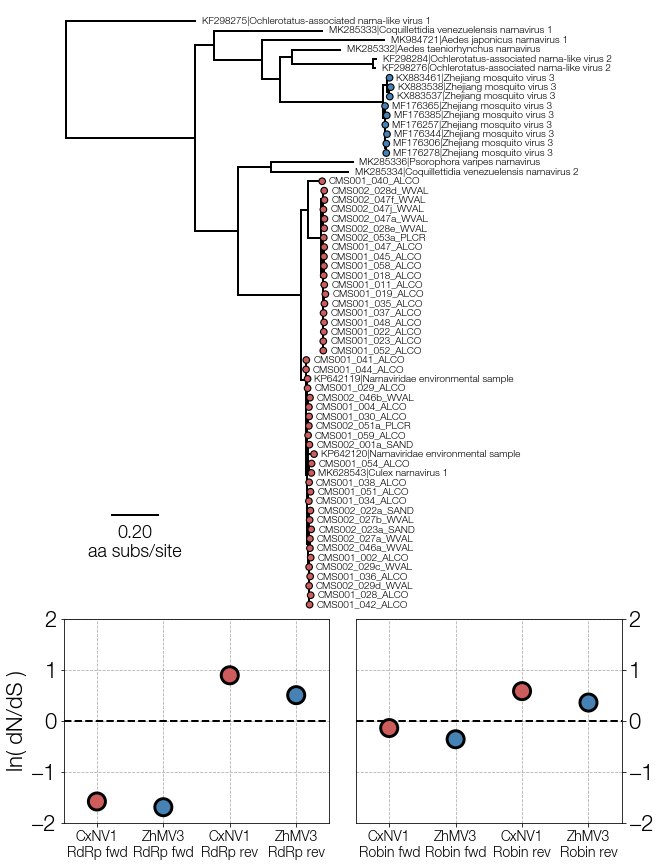
\includegraphics[width=0.5\textwidth]{narna-zhcx.png}
\caption{\label{fig: 1}
{\bf a} A maximum likelihood tree illustrating the relationship between CNV (\emph{Culex narnavirus 1}) (red) and
ZMV (\emph{Zheijiang mosquito virus 3}) (blue). {\bf b} ORF-wide dN/dS values for forward and reverse directions of RdRp and Robin segments for both viruses.
}
\end{center}
\end{figure}

Some careful consideration is required to reconcile our observations with results recently reported
in \cite{Ret+20}, where it was shown that introducing mutations which are non-synonymous on the reverse
open reading frame of Culex narnavirus 1 are able to reduce the fitness of this virus.
In the concluding section, we consider the interpretation of these observations, and discuss whether there
may be implications for other viral families.

There are many examples of overlapping viral genes with staggered reading frames: this was first
clearly described in \cite{Bar+76}, and has been reviewed in \cite{Chi+10}. Recent
work by Nelson, Ardern and Wei \citep{Nel+20} discusses how these can be identified.
Our investigations indicate that the ambigrammatic ORFs discussed in this work are a
different phenomenon, because they are non-coding. Our approach to analysing the ambigrammatic
sequences is quite distinct from the rather complex machinery proposed in \cite{Nel+20}, because
it emphasises the role of double synonyms as an unambiguous discriminant of the role of the ambigrammatic
sequences.

\section{Ambigram rules and their significance}
\label{sec: 2}

We start by describing the two genetic ambigram rules.

\begin{ambirule}All complementary-strand stops are removable \label{rule1}
\end{ambirule}

Consider the reading frame on the complementary strand that has its
codons aligned with those on the forward strand. Every codon on the forward
strand corresponds to a complementary-strand codon read in the reverse
direction. The rule states that any stop codon on the complementary strand
can be removed by a single-point mutation which leaves the amino acid specified by the
forward-read codon unchanged.

This result is demonstrated by the following argument, as discussed in \cite{DeR+19}. Reversing the read direction
and taking the pairing complement, the stop codons UAA, UAG, UGA in the standard genetic code become, respectively,
UUA, CUA, UCA, for which the amino acids are Leu, Leu, Ser. It is only instances of leucine and
serine in the forward sequence that can result in stop codons in the reverse read.
The synonyms of Leu are  CUN,  UUA, UUG (where N means any base).
The synonyms of Ser are UCN, AGU, AGC. The undesirable Leu codon UUA can be transformed
to UUG by a single substitution. Similarly, the Leu codon CUA can be transformed to
CUU, CUG or CUC by single substitutions. And the Ser codon UCA is transformed to UCU, UCG or UCC
by single substitutions. We conclude that every stop codon on the reverse reading frame can be removed
by a synonymous, single site nucleotide mutation.

Furthermore, it is found that complementary-strand stops cannot always be removed by synonymous substitutions
in the other two read frames for the complementary strand \citep[each case requires a separate and somewhat
involved argument, also given in][]{DeR+19}. As a consequence of these two arguments, we need discuss only the
complementary read frame with aligned codons.

\begin{ambirule}There exist double synonyms\label{rule2}
\end{ambirule}

Most synonymous mutations of the forward strand produce a non-synonymous change in the
complementary strand, but the genetic code does include a number of double synonyms,
where the reverse complement of a synonymous mutation is also a synonym.
For example codon AGG (Arg) can become CGG (Arg) via a synonymous mutation,
while the reverse complement of AGG, which is CCU (Pro) transforms to CCG (Pro) under
the same mutation.

The full set of double synonyms in the standard genetic code are as follows:

\begin{itemize}

\item Two of the six synonyms of Ser are double synonyms, with reverse complements coding Arg.
Conversely, two of the six synonyms of Arg are double synonyms, with reverse complement coding Ser.

\item Two more of the six synonyms of Arg are double synonyms, with reverse complement Pro.
Conversely, two of the four synonyms of Pro are double synonyms coding for Arg.

\item Two of the six synonyms of Leu are double synonyms, with reverse complement Gln.
Conversely, both synonyms of Gln are double synonyms, with reverse complement coding Leu.

\end{itemize}

Table \ref{tab: 1} lists the sets of single and double synonyms for those amino acids
that can have double synonyms. (We exclude the two synonyms of Ser and the one synonym
of Leu for which the reverse complement is Stop, because these do not occur in ambigrammatic
genes.)

\begin{table}[t]
\caption{For each amino acid (AA) that can have double-synonym mutations, we list
all of the possible codons which do not code for Stop on the complementary strand, indicating
their reverse complement (Comp. AA).
The codons that have a double synonym are marked with an asterisk.
For each of these codons, we list the number of mutations which are synonymous,
and the number of double synonym mutations. In each case the numbers of single (double) mutations are written
$S^{({\rm n})}+S^{({\rm v})}$ ($D^{({\rm n})}+D^{({\rm v})}$), where the superscript n denotes transitions,
and superscript v transversions. Also, double synonyms are counted in the list of single synonyms.
\label{tab: 1}}
\begin{tabular*}{\columnwidth}{@{\extracolsep\fill}clccc@{\extracolsep\fill}}
\toprule
AA&Codon&$S^{({\rm n})}+S^{({\rm v})}$&$D^{({\rm n})}+D^{({\rm v})}$&Comp. AA\\
\midrule
\multirow{4}{*}{Leu} &UUG$\ast$&$1+0$&$1+0$&Gln\\
       &CUU&$1+1$&$0+0$&Lys\\
       &CUC&$1+1$&$0+0$&Glu\\
       &CUG$\ast$&$1+2$&$1+0$&Gln\\
\midrule
\multirow{4}{*}{Pro} &CCU$\ast$&$1+2$&$0+1$&Arg\\
       &CCC&$1+2$&$0+0$&Gly\\
       &CCA&$1+2$&$0+0$&Trp\\
       &CCG$\ast$&$1+2$&$0+1$&Arg\\
\midrule
\multirow{2}{*}{Gln} &CAA$\ast$&$1+0$&$1+0$&Leu\\
       &CAG$\ast$&$1+0$&$1+0$&Leu\\
\midrule
\multirow{6}{*}{Arg} &CGU&$1+2$&$0+0$&Thr\\
       &CGC&$1+2$&$0+0$&Ala\\
       &CGA$\ast$&$1+3$&$0+1$&Ser\\
       &CGG$\ast$&$1+3$&$0+1$&Pro\\
       &AGA$\ast$&$1+1$&$0+1$&Ser\\
       &AGG$\ast$&$1+1$&$0+1$&Pro\\
\midrule
\multirow{5}{*}{Ser} &UCU$\ast$&$1+1$&$0+1$&Arg\\
       &UCC&$1+1$&$0+0$&Gly\\
       &UCG$\ast$&$1+2$&$0+1$&Arg\\
       &AGU&$1+0$&$0+0$&Thr\\
       &AGC&$1+0$&$0+0$&Ala\\
\botrule
\end{tabular*}
\end{table}

\subsection{Implications}
\label{sec: 2.3}

Our first rule shows that an ambigrammatic version of any gene can evolve, without
making any changes to the amino acid sequence. This establishes how ambigrammatic sequences
can arise, but it does not illuminate why they are favoured.

Combined with observed polymorphisms of narnaviruses, the second ambigram rule can give an
indication of the utility of ambigrammatic sequences. In studies on the (usual) non-ambigrammatic
genomes, the ratio of synonymous to non-synonymous mutations is used as an indicator of
whether the nucleotide sequence codes for a protein: non-synonymous mutations
are likely to be deleterious if the sequence codes for a functional protein.
We shall adapt this approach to our study of ambigrammatic narnavirus genes.
We assume that the forward direction is a coding sequence (usually for RdRp),
and confine attention to those mutations which are synonymous in the forward
direction. If the complementary strand codes for a functional protein, most of these
synonymous mutations will inevitably result in changes of the complementary
amino acid sequence. However, at many loci the evolutionarily favoured amino acid
will be one that allows double synonyms. In these cases, there can be
non-deleterious mutations between a pair of codons that preserve the amino acid
sequence of both the forward and the
complementary strands.

If the complementary strand codes for a functional protein, we expect studies of the
polymorphism of the gene would show that these double-synonym loci will be
mutational \lq hotspots', where mutations occur more frequently. In addition, the double-synonym pairs
would be represented far more frequently than other mutations at these loci. These observations
lead to two distinct tests for whether there is evolutionary pressure on the translated sequence of the
complementary strand.

\section{Ambigrammatic narnavirus genes}
\label{sec: 3}

We analysed data from samples of two ambigrammatic narnaviruses,
\emph{Culex narnavirus 1} (CNV, with $46$ genomes) and \emph{Zhejiang mosquito virus 3} (ZMV, with
$10$ genomes). Both narnaviruses have an ambigrammatic RdRp coding gene, denoted CNV-RdRp and
ZMV-RdRp respectively. The reverse open reading frame has its codons aligned with the forward frame.
In both forward and reverse reading frames any stop codons are close to the end $3'$ end of the
respective frame.

The ambigrammatic feature is certainly a puzzle. There appear to be two classes
of plausible of explanation:

\begin{enumerate}

\item {\bf The reverse open reading frame codes a protein}. This is logically possible, but
if the RdRp gene is strongly conserved, there is very little flexibility in the rORF. However, in the
absence of any additional evidence it is the explanation which requires the fewest additional hypotheses.

\item {\bf The reverse open reading frame facilitates association of ribosomes with RNA}. This
could conceivably convey advantages by providing a mechanism to protect viral RNA from
degradation, but without additional evidence this requires additional hypotheses.

\end{enumerate}

Recently, additional evidence has emerged which may provide support for the second of these explanations.
Specifically, the CNV infection has recently been shown to be facilitated by another ambigrammatic viral
RNA segment, termed \emph{Robin} (\cite{Bat+20,Ret+20}). It was reported that this segment, CNV-Robin,
is ambigrammatic, with forward and reverse codons aligned, over very nearly
the entire length (about $850{\rm nt}$), where direction designation is determined by which amino acid sequence appears more conserved. Again, any stop codons occur close to the $3'$ end.
Neither forward nor reverse directions of Robin are homologous with known sequences.

Because ambigrammatic genes are rare, finding two of them in the same system is a strong
indication that their occurrence has a common explanation. This observation makes it
appear unlikely that the reverse open reading frame is a device to \lq pack in' an additional
protein coding gene, and more likely that the ambigrammatic feature is associated with
allowing ribosomes to associate with both strands of the viral RNA.

This reasoning suggests that the Robin gene may play a role in selecting for the
ambigrammatic property (for example, it may facilitate viral RNA being protected
by ribosomes). If this surmise is correct, we should expect to see a version of the Robin
gene associated with other ambigrammatic narnaviruses. It is possible that this might be detected
by a search of archived sequence data. Only Zhejiang mosquito virus 3 appeared to
be observed multiple times to make detection of an additional Robin segment possible, so we
concentrated on that system.

We were able to find evidence of an ambigrammatic RNA, of length
approximately $900{\rm nt}$, that co-occurs with ZMV RdRp segment across multiple samples recovered by at least two studies that, like CNV Robin, bears no recognisable homology to publicly available sequences or CNV Robin itself.
Given the conjunction of these unusual features we strongly believe this ambigrammatic RNA to be the equivalent of a Robin segment in ZMV.

\section{Tests of whether the complementary strand is coding}
\label{sec: 4}

We have argued that doubly-synonymous mutations will give a signature of the
reverse strand coding for a functional protein. If the reverse-direction code is functional,
then the only assuredly non-deleterious mutations would be the double-synonym ones,
where one codon is transformed by a single-nucleotide substitution to another
codon which preserves the amino acid coded in both the forward and
the reverse directions.

Assume that we have $M$ sequences of an ambigrammatic gene, fully sequenced and
maximally aligned with each other, and that one strand, referred to as the
\lq forward' strand, codes for a functional protein.
We identify a \lq consensus' codon at each of the $N$ loci,
and then enumerate the set of variant codons at each amino acid locus.
If the consensus codon at a locus is one of the twelve
double-synonym codons listed in table \ref{tab: 1}, we term this a \emph{doubly-synonymous locus}.
The number of doubly-synonymous loci is $N_{\rm ds}$.

There are two different approaches to testing whether
double synonyms indicate that the complementary strand is coding:

\subsection{Look for the existence of mutational \lq hotspots'}
\label{sec: 4.1}

We can look for evidence that the doubly-synonymous loci experience more substitutions than other loci.

For each codon locus $k$, we can determine the number of elements of the variant set, $n(k)$,
and also the fraction of codons $f(k)$ which differ from the consensus codon.
We then determine the averages of these quantities, $\langle n(k)\rangle$ and $\langle f(k)\rangle$,
for the doubly-synonymous loci and for the other loci. If the ratios
%
\begin{equation}
\label{eq: 4.1}
R_n=\frac{\langle n(k)\rangle\vert_{\rm double\ syn.\ loci}}{\langle n(k)\rangle\vert_{\rm other\ loci}}
\ ,\ \ \
R_f=\frac{\langle f(k)\rangle\vert_{\rm double\ syn.\ loci}}{\langle f(k)\rangle\vert_{\rm other\ loci}}
\end{equation}
%
are large, this is evidence that the complementary strand is coding.

The null hypothesis, indicating that the reverse open reading frame is
non-coding, is that the ratios $R_n$ and $R_f$ are sufficiently close to
unity that the difference may be explained by statistical fluctuations.

\subsection{Mutation frequencies test}
\label{sec: 4.2}

We can also look at codon frequencies for different mutations at doubly-synonymous loci.
If the complementary strand is coding, we expect to find that the frequency of mutations
observed at doubly-synonymous loci will heavily favour double-synonym codons over
single synonyms.  We consider the subset of double-synonym loci where mutations
are observed (that is, where $n(k)>1$). For each of these $N_{\rm a}$ \emph{variable doubly-synonymous loci}, we can determine two numbers: $n_{\rm s}(k)$ is
the numbers of singly-synonymous variants at locus $k$, and $n_{\rm d}(k)$ is the number
of these variants which are also doubly-synonymous. (Clearly $n(k)\ge n_{\rm s}(k)\ge n_{\rm d}(k)$).
If $n_{\rm d}(k)=n_{\rm s}(k)$, that means that the mutations preserve the complementary-strand
amino acid, which is an indication that the reverse strand is coding. If $\{k^\ast\}$
is the set of variable doubly-synonymous loci, we then
calculate
%
\begin{equation}
\label{eq: 4.2}
N_{\rm s}=\sum_{k\in\{k^\ast\}} n_{\rm s}(k)
\ ,\ \ \
N_{\rm d}=\sum_{k\in\{k^\ast\}} n_{\rm d}(k)
\ .
\end{equation}
%
If the complementary strand is coding, we expect
%
\begin{equation}
\label{eq: 4.3}
R\equiv \frac{N_{\rm s}}{N_{\rm d}}
\end{equation}
%
to be close to unity.

However, there will also be beneficial
or neutral mutations which do change the amino acids, so that not all mutations
will be between sets of doubly-synonymous codons. We need to be able to
quantify the extent to which finding other than double-synonym mutations is
an indication that the reverse strand is non-coding. We must do this by comparison with
a null hypothesis, in which the reverse strand is non-coding.

\subsection{Null hypothesis for mutation frequencies}
\label{sec: 4.3}

Let $R_0$ be the value of the ratio $R$ that is derived from this null hypothesis that
the complementary strand is non-coding.
In order to compute the expected $N_{\rm s}/N_{\rm d}$ ratio, $R_0$, we adopt the following
approach. We assume that the $M$ sequences are sufficiently similar
that only a small fraction of loci have undergone mutations.
We adopt the Kimura model \citep{Kim80}, which assumes that the mutation
rates for transitions (${\rm A}\leftrightarrow {\rm G}$ or ${\rm C}\leftrightarrow{\rm U}$) are
different from those of transversions (other single-nucleotide mutations), and negligible for
other types of mutation. The ratio of these rates is
%
\begin{equation}
\label{eq: 6.6}
\alpha=\frac{r_{\rm trn}}{r_{\rm trv}}
\ .
\end{equation}
%
If the numbers of single (double) synonyms of the consensus nucleotide at locus $k$ leading to
transitions or transversions are respectively $S^{({\rm n})}_k$ and $S^{({\rm v})}_k$
($D^{({\rm n})}_k$, $D^{({\rm v})}_k$), then we estimate
%
\begin{equation}
\label{eq: 4.7}
R_0=
\frac{\sum_{k\in\{k^\ast\}}\alpha S_k^{({\rm n})}+S^{({\rm v})}_k}
{\sum_{k\in\{k^\ast\}}\alpha D^{({\rm n})}_k+D_k^{({\rm v})}}
\end{equation}
%
The numbers $S^{({\rm n})}_k$, $S^{({\rm v})}_k$, $D^{({\rm n})}_k$, $D^{({\rm v})}_k$ are given
in table \ref{tab: 1} for all of the double-synonym codons.

\subsection{Finding the Robin segment of Zhejiang mosquito virus 3}

We looked through assembled contig datasets from two metagenomic mosquito studies (three from China and six from Australia)\cite{shi_16,shi_17}, kindly provided to us by Mang Shi and Edward C Holmes.
We clustered contigs from the nine datasets by similarity using CD-HIT\cite{fu_12} with a threshold of 90\% and looked for clusters that contained contigs from at least $6$ samples, that did not have standard deviation in contig length greater than $1 200$, and had fewer than $200$ contigs.
Of the hundreds of clusters filtered this way only a handful also possessed sequences ambigrammatic across at least 90\% of their length and only two clusters were mostly comprised of ambigrammatic sequences, while the rest were clearly recognisable as mosquito contigs.
Of the two clusters one was identifiable as the RdRp of Zhejiang mosquito virus 3, while we presume the other to be an unrecognisably distant orthologue of Culex narnavirus 1 Robin, on account of its co-occurrence with ZMV RdRp, ambigrammaticity, and length.

ORF-wide dN/dS values were computed by assuming that every mutation in the alignment has occurred only once to be conservative. This was motivated by the presence of pairs of sites with four haplotypes between them ($4$G sites), an indication that recombination may be a potential issue with narnavirus sequences.
Normalising the number of observed non-synonymous and synonymous mutations was done by assuming a transition/transversion ratio of $2$.


\section{Results}
\label{sec: 5}

Next we report the results of our studies of polymorphism of the four ambigrammatic narnavirus genes.
We discuss what can be learned from applying standard techniques, before discussing
the results of our tests for whether the reverse open reading frame codes for a protein.

\subsection{Forward reading frame}
\label{sec: 5.1}

Each sequence was trimmed to a length of $3N$ nucleotides. We identified a consensus
nucleotide at each locus, and determined the set of variant nucleotides at each locus.
We determined the total number of transition and transversion mutations which are observed,
$N_{\rm trn}$ and $N_{\rm trv}$ respectively. We also determined the total number
of mutations at each position in the codon, $(n_1,n_2,n_3)$.
We estimated the average number of variable sites $r$ as the total number of nucleotide variants,
divided by the product of the number of sequences and alignment length. We also
estimated the ratio $\alpha$ of the rate of selected transition mutations to the rate of transversions:
%
\begin{equation}
\label{eq: 5.1}
r\equiv \frac{n_1+n_2+n_3}{3NM}
\ ,\ \ \
\alpha\equiv \frac{r_{\rm trn}}{r_{\rm trv}}=\frac{2N_{\rm trn}}{N_{\rm trv}}
\end{equation}
%
(recall that there are twice as many transversions as transitions). We also determined a \lq normalised'
triplet of variable sites for each position within the codon: $(z_1:z_2:z_3)=3(n_1:n_2:n_3)/(n_1+n_2+n_3)$.
Our results on the nucleotide-level
investigation of polymorphism are summarised in table \ref{tab: 5.1}.

We then assigned a consensus codon at each codon locus, selecting the
frame by the criterion of minimising the number of stop codons.
For each of the $N$ codons, we determined the variant set of codons
which were observed in each of the $M$ sequences. The total
number of synonymous and non-synonymous single-nucleotide changes in the variant sets
was $N_{\rm s}$ and $N_{\rm ns}$ respectively. The total number of mutations
encountered in the variant sets where two or three nucleotides were changed was $N_{\rm mult}$.
For each codon there are
numbers of possible non-synonymous mutations which are transistions and transversions,
$n_k^{({\rm trn})}$ and $n_k^{({\rm trv})}$, and numbers of synonymous mutations
which are transitions and transversions, $s_k^{({\rm trn})}$ and $s_k^{({\rm trn})}$
(with $s_k^{({\rm trn})}+n_k^{({\rm trn})}+s_k^{({\rm trv})}+n_k^{({\rm trv})}=9$). Under the null
hypothesis that the sequence is non-coding, the expected value of the ratio
%
\begin{equation}
\label{eq: 5.2}
R=\frac{N_{\rm ns}}{N_{\rm s}}
\end{equation}
%
is
%
\begin{equation}
\label{eq: 5.3}
R_0=\frac{\sum_{k=1}^N\alpha n_k^{({\rm trn})}+n_k^{({\rm trv})}}
{\sum_{k=1}^N\alpha s_k^{({\rm trn})}+s_k^{({\rm trv})}}
\ .
\end{equation}
%
We also determined the fraction of codons where multi-nucleotide mutations are observed,
$f_{\rm mult}=N_{\rm mult}/N$.
We present our results for the codon-level mutations in table \ref{tab: 5.2}, which includes information
for both the forward and the complementary read directions (with codon boundaries aligned
for the complementary direction).

The alignments are \emph{ambigrammatic}, in the sense that there are no stop codons in the
interior of the sequence. None of the individual sequences had stop codons in the body of the
sequence in either direction.

Based upon these tables, we can make the following observations and deductions:

\begin{enumerate}

\item{\bf Diversity}. We observe that both RdRp and Robin
segments are comparable in their diversity, for both CNV and ZMV.
As expected, RdRp sequences are highly conserved at the amino acid level.
Robin, on the other hand, appears far more relaxed at the amino acid level and, consistent with this, diverged beyond recognition between CNV and ZMV.

\item{\bf Relative mutation rate by codon position}. For RdRp sequences, more mutations are observed
at the third nucleotide in each codon, as expected for a sequence that preserves the amino acid sequence
(because most synonymous mutations involve the third nucleotide of a codon). In the case of Robin sequences,
the frequencies of mutation are much closer to being equal, to the extent that for CNV-Robin the null hypothesis
that the rates are equal is not definitively rejected. However, mutations at different
codon sites are sufficiently weighted towards the third position that we shall assume that Robin
does code for a functional protein.

While the values of $(z_1:z_2:z_3)$ are very different for RdRp and Robin, their values are
comparable for CNV and ZMV, which is an indication that the selective pressures on both
viruses are the same.

\item{\bf Rate of multiple nucleotide mutations}. The fraction of multiple nucleotide mutations is
higher for Robin sequences than it is for RdRp sequences.

\item{\bf Transition to transversion ratio}. Three of the values of $\alpha$ were similar to each other, while the value
for ZMV-RdRp was higher than the others. Because transitions occur at a higher intrinsic rate, a lower
value of $\alpha$ indicates that observed mutations are biased in favour of the rarer transversions,
which is an indication of unusual selective pressures. The fact that the values of $\alpha$ for the Robin segments are
comparable to, or lower than, the values for RdRp are a further indication that Robin
is under similar selective pressure too.

\item{\bf Ratio of non-synonyms to synonyms}. For the RdRp segments the values of
$R=N_{\rm ns}/N_{\rm s}$ are much smaller than the values $R_0$
predicted (equation (\ref{eq: 5.3})) by the null hypothesis that mutations are random. This indicates that the selective
pressure on RdRp acts to preserve the amino acid sequence. For Robin segments, the values of $R$
are much larger, but still smaller than the prediction from the null hypothesis. This indicates that while
points 1-4 above indicate that Robin is under some selective pressure, the amino acid sequence
is not strongly conserved.
This is consistent with the hypothesis that the selection acting on Robin is relaxed.

\end{enumerate}

Figure \ref{fig: 2} illustrates the distribution of mutations across the forward and reverse reading frames
of all four ORFs for both CNV and ZMV. As expected, there is evidence that some regions accumulate mutations more readily than others.
The pattern is consistent with what would be expected from the statistical reductions in the tables.

\begin{figure*}
\begin{center}
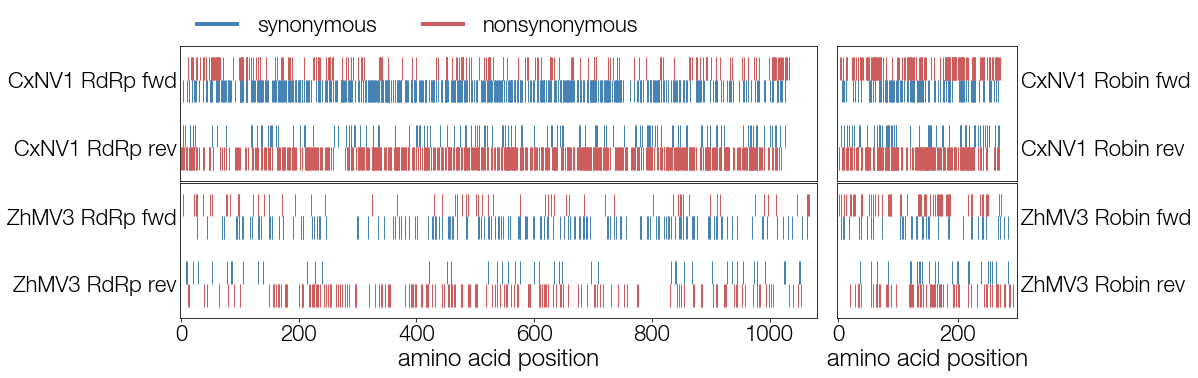
\includegraphics[width=0.9\textwidth]{narna-diversity.png}
\caption{\label{fig: 2}
Distribution of synonymous (blue) and non-synonymous (red) substitutions in CNV (upper plots) and ZMV (lower plots) RdRp (left) and Robin (right) segments in both directions (forward towards top, reverse towards bottom).
Translated ORFs are shown in their own coordinate space, rather than with respect to their position in the segment.
}
\end{center}
\end{figure*}

\begin{table*}
\centering
\begin{tabular}{|c|c|c|c|c|c|c|c|c|}
\hline
Strand&$N$&$M$&$N_{\rm trn}$&$N_{\rm trv}$&$r$&$\alpha$&$(n_1,n_2,n_3)$&$(z_1:z_2:z_3)$\\
\hline
CNV-RdRp&$1033$  &$46$ &$606$ &$362$&$0.0068$&$3.35$ &$(181,140,645)$&$(0.56:0.44:2.00)$\\
ZMV-RdRp&$1075$ &$12$&$210$ &$39$& $0.0064$ &$10.8$ &$(47,29,173)$&$(0.57:0.35:2.08)$\\
CNV-Robin&$272$    &$46$ &$213$ &$146$&$0.0096$&$2.92$ &$(107,100,152)$&$(0.89:0.84:1.27)$\\
ZMV-Robin&$304$&$10$&$84$&$48$&$0.0145$&$3.50$&$(35,31,66)$&$(0.80:0.70:1.50)$\\
\hline
\end{tabular}
\caption{
\centering
Nucleotide-level statistics of mutations.
\label{tab: 5.1}}
\end{table*}

\begin{table*}
\centering
\begin{tabular}{|c|c|c|c|c|c|c|c|}
\hline
Strand&$N_{\rm s}$&$N_{\rm ns}$&$N_{\rm mult}$&$R=N_{\rm ns}/N_{\rm s}$&$R_{\rm exp}$
&$R/R_0$&$f_{\rm mult}$\\
\hline
CNV-RdRp-fwd   &$623$ &$189$ & $123$ &$0.303$ &$2.37$&$0.128$&$0.12$\\
ZMV-RdRp-fwd   &$170$ &$59$ & $13$ &$0.347$ &$2.14$&$0.162$&$0.012$\\
CNV-Robin-fwd   &$112$&$141$& $89$   &$1.26$ & $2.34$&$0.538$&$0.45$\\
ZMV-Robin-fwd   &$49$&$61$& $14$   &$1.24$ & $2.35$&$0.528$&$0.046$\\
CNV-RdRp-comp &$136$&$676$& $123$ &$4.97$ &$2.43$&$2.04$&$0.12$\\
ZMV-RdRp-comp &$50$&$179$& $13$ &$3.58$ &$2.14$&$1.67$&$0.012$\\
CNV-Robin-comp &$66$&$187$&$89$&$2.83$&$2.39$&$1.23$&$0.45$\\
ZMV-Robin-comp &$32$&$78$&$14$&$2.43$&$2.28$&$1.07$&$0.046$\\
\hline
\end{tabular}
\caption{
\centering
Summary of results for codon-level mutations.
\label{tab: 5.2}}
\end{table*}

\subsection{Complementary reading frame}
\label{sec: 5.2}

We determined the set of $N_{\rm d}$ doubly-synonymous codons in the consensus sequence, and
the subset of $N_{\rm a}$ of these which have variant codons.

\begin{enumerate}

\item{\bf Mutational hotspots test}. We applied the mutational hotspots test to all four sequences,
as described by equations (\ref{eq: 4.2}) and (\ref{eq: 4.3}) above.
The results (tables \ref{tab: 5.4}) show no evidence that the doubly synonymous sites are
undergoing more frequent mutations, or that their mutations are more widely spread across the dataset.

\item{\bf Mutation rate test}. We examined the number of mutations in the set
of $N_{\rm a}$ doubly-synonymous sites which were variable. We found (table \ref{tab: 5.5})
that many more of the observed mutations at these sites are only singly synonymous, when
a doubly-synonymous mutation is possible, which is further evidence that the complementary
strand is non-coding. The numbers of doubly-synonymous mutations
were quite low, and so it was not possible to make a reliable comparison of the
ratio $N_{\rm s}/N_{\rm d}$ with the null hypothesis.

\item{\bf Ratio of non-synonyms to synonyms}.

The ratios of non-synonymous to synonymous mutations, presented in table \ref{tab: 5.2}, were
lower than the null-hypothesis for the forward direction. This is readily explained as an indication
that the forward ORF codes for a functional protein. However the $N_{\rm ns}/N_{\rm s}$
ratios for the reverse direction were all higher than the null hypothesis. This observation
is explained, qualitatively, as follows.
If the forward direction strictly conserves the amino acid sequence, then all of the mutations
which are synomymous on the reverse strand are doubly-synonymous. Because only
$12$ of the $64$ codons allow for doubly-synonymous mutations, the $N_{\rm ns}/N_{\rm s}$
ratio would be very high for the complementary strand if the forward sequence were to be exactly conserved.
We computed this ratio, and found $11.2$ for CNV-RdRp, and similar values for the other sequences.
This theoretical ratio is considerably higher than the measured value of $4.97$, because the
forward sequence is not exactly conserved. For Robin segments, the value of $R$ for the reverse
ORF is only slightly higher than the null hypothesis, because the amino acid sequence is only weakly
conserved.

\end{enumerate}


\begin{table*}[h]
\begin{minipage}{0.5\textwidth}
\centering
\begin{tabular}{|c|c|c|}
\hline
Sample&$\langle n(k)\rangle$&$\langle f(k)\rangle$\\
\hline
Double syns., CNV-RdRp  &$0.954$&$0.161$\\
Other codons, CNV-RdRp  &$0.968$&$0.155$\\
Double syns., ZMV-RdRp  &$1.20$&$0.042$\\
Other codons, ZMV-RdRp  &$1.23$&$0.050$\\
Double syns, CNV-Robin &$1.76$&$0.195$\\
Other codons, CNVRobin &$1.48$&$0.169$\\
Double syns, ZMV-Robin   &$0.889$&$0.096$\\
Other codons, ZMV-Robin &$0.960$&$0.097$\\
\hline
\end{tabular}
\end{minipage}
\begin{minipage}{0.4\textwidth}
\centering
\begin{tabular}{|c|c|c|c|c|}
\hline
Gene&$N$&$N_{\rm ds}$&$R_n$&$R_f$\\
\hline
CNV-RdRp  &$1033$&$220$&$0.986$&$1.044$\\
ZMV-RdRp  &$1075$&$219$&$0.975$&$0.840$\\
CNV-Robin  &$272$&$54$&$1.19$&$1.16$\\
ZMV-Robin  &$304$&$81$&$0.926$&$0.978$\\
\hline
\end{tabular}
\end{minipage}
\caption{Summary of results of \lq mutational hotspots' test. Left panel: values of the average number
of elements of the variant set, $\langle n(k)\rangle$ and of the average fraction of non-consensus
codons, $\langle f(k)\rangle$, for double-synonym sites,  and for the other sites.
Right panel: $N$ is the number of loci in the alignment, $N_{\rm ds}$ is the
number of double-synonym loci, and $R_n$, $R_f$ are the ratios of $\langle n(k)\rangle $
and $\langle f(k)\rangle$ at double-synonym sites to their values at other sites.
The differences of these ratios from unity do not appear significant.
\label{tab: 5.4}}
\end{table*}

\begin{table}
\centering
\begin{tabular}{|c|c|c|c|c|c|c|c|c|}
\hline
Sample&$N$&$N_{\rm a}$&$N_{\rm s}$&$N_{\rm d}$&$R$&$R_0$&$R/R_0$\\
\hline
CNV-RdRp  &$1033$&$136$&$151$&$60$&$2.51$&$3.02$&$0.83$\\
ZMV-RdRp  &$1075$&$219$&$33$&$20$&$1.65$&$3.21$&$0.51$\\
CNV-Robin  &$272$&$40$&$24$&$3$&$8.00$&$3.21$&$2.49$\\
ZMV-Robin  &$304$&$59$&$20$&$4$&$4.00$&$4.04$&$0.99$\\

\hline
\end{tabular}
\caption{Results for the mutational codon frequency test: $N$ is the number of loci
in the alignment, $N_{\rm a}$ is the number of mutationally active double-synonym loci, and
$N_{\rm s}$, $N_{\rm d}$ are, respectively, the numbers of single and double synonym mutations.
\label{tab: 5.5}}
\end{table}

\section{Discussion}
\label{sec: 6}

We have argued that doubly synonymous codons provide a key to understanding whether
ambigrammatic viral RNA segments code for two functional proteins. If there were two
coding genes, doubly synonymous mutations would be mutational hotspots,
because they are unambiguously non-deleterious. We applied our analysis to recent
observations of polymorphisms in two ambigrammatic narnaviruses: Culex narnavirus 1
and Zhejiang mosquito virus 3. There was no evidence that doubly synonymous
sites are mutational hotspots, or that there is a prevalence of mutations to other doubly-synonymous codons
at these sites. Other, circumstantial, evidence favours the interpretation that the complementary strand is non-coding.
Ambigrammatic sequences have been observed in other narnaviruses,
but they are undoubtedly a rare phenomenon.
If the rORF (reverse open reading frame) of both RdRp and Robin segments
had evolved to code for a functional protein, each RNA segment would code for two genes.
Given that ambigrammatic sequences are rare \citep{DeR+19}, finding a system where two had evolved
independently would be highly improbable. Moreover, because the ambigrams are full length,
each of the ambigrammatically coded sequences would code for two genes which have the same
length as each other.

An observation of the simultaneous detection of two or more ambigrammatic genes would
strongly favour models where there is an advantage in evolving an
ambigrammatic sequence which is independent of whether the reverse open reading
frames are translated into functional proteins. This argument led us to discover the Robin segment
of ZMV, and suggests that more ambigrammatic narnaviruses with at least two segments will be discovered
by metagenomic surveys, when suitable data sets become available.
Similarly, the elusive Robin segment should already be hiding in datasets of narnaviruses descended from the common ancestor of CNV and ZMV.


Our studies of polymorphisms in the forward direction indicate that both RdRp and Robin are under purifying selection.
In the case of RdRp the amino acid sequence is strongly conserved,
but the Robin sequence isn't.

The role of the RdRp coding fragment
is already understood. This makes it plausible that the other fragment plays a role which facilitates the
evolution of ambigrams. If the lack of stop codons on the complementary strand is not required
to allow protein synthesis, we can surmise that its role is to allow ribosomes to associate with the
complementary strand. Having RNA segments able to be covered by ribosomes may provide some protection
for the viral RNA against degradation.

The role of Robin is uncertain. Ribosome profiling suggests that most of the ribosomes attached to
the viral RNA become stalled, creating a cover \cite{Cep20,Ret+20,Wil+21}. The ambigram property
allows binding of ribosomes to both strands, hiding the viral RNA from host defence and degradation mechanisms.
It is possible that Robin plays a role in this process, possibly by creating a protein which
blocks ribosome detachment at $3'$ end. Without a better understanding of the narnavirus lifecycle in arthropods
alternative functions for the Robin protein may also be viral suppression of RNAi\cite{mie_14} or formation of syncytia or viral particles.

It might be proposed that the ribosome \lq traffic jam' is a consequence of the structure of the
RdRp itself, possibly due to formation of RNA hairpins. However, these would have to trade off against RdRp function.
The proposed mechanism involving Robin making a blocking protein
has the advantage that the RdRp works efficiently when the viral RNA concentration is small.
Later, after it has duplicated many copies of itself and of Robin, the Robin protein attaches
to the viral RNA and creates stalled polysomes, protecting the viral RNA from degradation.

One aspect of this picture which requires refinement is that stalled ribosomes are usually detached
by \lq no-go-decay'. Another viral gene may be required to disrupt this process. We searched
for an additional ambigrammatic gene, so far without success. In fact it is possible that \lq Robin'
is the gene which disrupts \lq no-go-decay', and that it is the gene for blocking ribosome detachment
which is still to be identified.

Further studies of \lq ribosome profiling' of this system have the potential to reveal evidence
of whether ribosomes accumulate on the viral RNA in this system.  A recent preprint \citep{Ret+20}
presents evidence that inserting mutations in the RdRp sequence which are synonymous in the forward
reading frame but introduce stop codons in the reverse frame reduces the fitness of the virus. The mutations
were clustered close to the $3'$ end of the RdRp gene. These
observations could be interpreted as indicating that the reverse reading frame codes for a functional
protein or that all ORFs in the cell may be translated in a \lq leaky' way.
However, changing the RNA sequence may also interfere with the action of molecules which
bind to the RdRp strand.


\section{Competing interests}
There is NO Competing Interest.

\section{Author contributions}

GD devised and directed the search for an analog of Robin in the ZMV sequence
archive. MW produced a draft of the manuscript following discussions with the other
authors about the recent discovery of a narnavirus system which has two
ambigrammatic genes. All authors contributed to writing the manuscript, and
reviewed the manuscript before submission.


\section{Acknowledgments}

We thank Hanna Retallack and Joe DeRisi for discussions of their experimental studies of narnaviruses
and Amy Kistler for assistance with narnaviral genomes.
We would like to thank Mang Shi and Edward C Holmes for sharing assembled contigs from Australian and Chinese mosquito metagenomic datasets.
G.H. and D.Y. were supported by the Chan Zuckerberg Biohub;
MW thanks the Chan Zuckerberg Biohub for its hospitality.

\section{Data availability}


%USE THE BELOW OPTIONS IN CASE YOU NEED AUTHOR YEAR FORMAT.
\bibliographystyle{abbrvnat}

\bibliography{polyvirus}

%USE THE BELOW OPTIONS IN CASE YOU NEED NUMBERED FORMAT. UNCOMMENT THE ABOVE TWO LINES.
%\bibliographystyle{plain}
%\bibliography{reference}




\end{document}
